\subsection{Replacement Strategy}
Due to the lifespan of the CubeSats, the whole constellation is replaced every five years, hence, a replacement strategy has to be designed. As stated in the First Placement section, the orbital planes are deployed consecutively, thus, the replacement has to be so also. One simple solution could be waiting for a plane to de-orbit and then place a new one into the same position, however, this procedure would spend to much time by the fact that the satellites approach the atmosphere in a very slow rate. Additionally, the replacement of different planes would probably overlap. Since the first placement has been carefully designed, it is thought to adapt the same procedure to the replacement process, that means, to consider the replacements as a first placement. Obviously, some differences have to be taken into account given that at this point there is a constellation providing full service to the customers. The problem remains on the fact that in order to use the same strategy, the replacement needs to be achieved in eight weeks, therefore, the new orbital planes cannot be situated into the same position than the old ones. A rapid replacement is also interesting regarding the need of providing full service to the customers without interruption. The solution adopted consists on placing the new planes between the old ones consecutively, following the order of the first placement. In order to clarify the process, a detailed explanation is shown below:
\newline\newline
First of all, since different orbital planes are going to be taken into account in this explanation a nomenclature is set: old planes are the ones that have to be replaced, the new ones are the planes that will substitute them. If a plane is named with the number 1, it means that is the first one to be placed (old or new) and so on (2,3,..,21). 
\begin{itemize}
\item The new plane 1 is placed between the old plane 1 and the old plane 21.
\item The new plane 2 is placed between the old plane 1 and the old plane 2 to ensure that at the very moment the first old plane begins to decay, it does not appear a gap.
\item At this point, the following new planes are deployed consecutively between the old ones until the constellation is fully renovated. This maneuver is repeated every five years to ensure the continuity of the Astrea Constellation. 
The following images show the process explained above.
\end{itemize}
\begin{figure}[h!]
\centering 
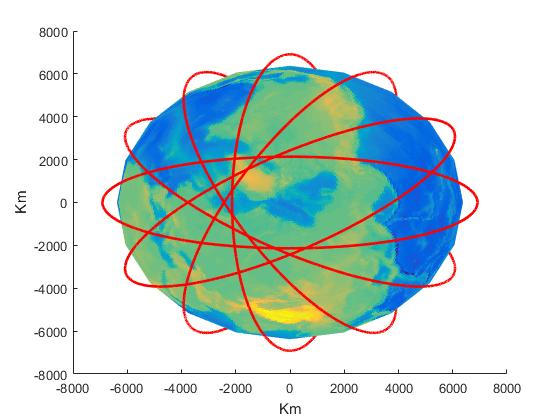
\includegraphics[scale=0.7]{./sections/Constellation_Deployment/S5-1-Replacement_Strategy/Images_S5-1/Picture_1_S5-1.jpg} 
\caption{Old Constellation}
\label{fig:rp1}
\end{figure}

\begin{figure}[h!]
\centering 
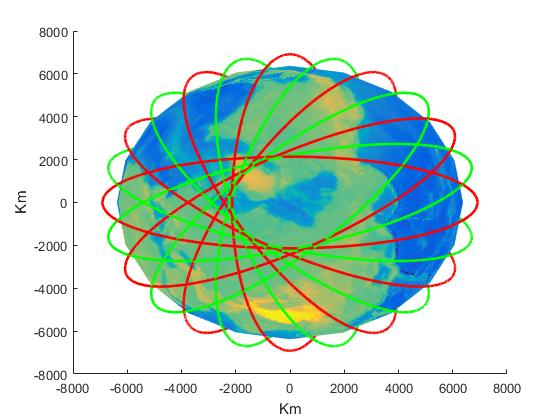
\includegraphics[scale=0.7]{./sections/Constellation_Deployment/S5-1-Replacement_Strategy/Images_S5-1/Picture_2_S5-1.jpg} 
\caption{Old and New Constellations}
\label{fig:rp2}
\end{figure}

\begin{figure}[h!]
\centering 
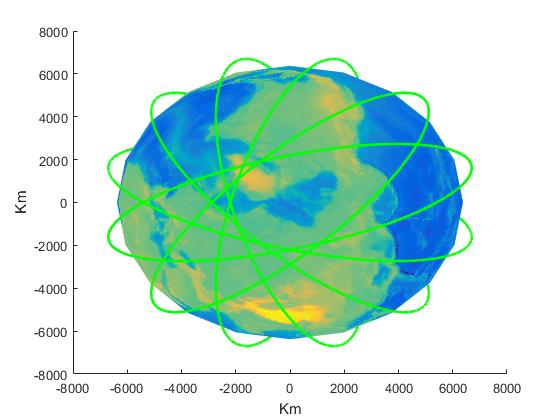
\includegraphics[scale=0.7]{./sections/Constellation_Deployment/S5-1-Replacement_Strategy/Images_S5-1/Picture_3_S5-1.jpg} 
\caption{New Constellation}
\label{fig:rp3}
\end{figure}

